\documentclass[12pt, a4paper]{article}
\usepackage[utf8]{inputenc}
\usepackage[T1]{fontenc}
\usepackage[brazilian]{babel}
\usepackage[top=3cm, bottom=2cm, left=3cm, right=2cm]{geometry}
\usepackage{times}
\usepackage{setspace}
\usepackage{graphicx}
\usepackage{indentfirst}
\usepackage{booktabs}
\usepackage{tabularx}
\usepackage{amsmath}
\usepackage{amsfonts}
\usepackage{float}
\usepackage{caption}
\usepackage[alf, abnt-emphasize=bf]{abntex2cite}
\doublespacing
\captionsetup[figure]{skip=2pt, font=small, labelfont=bf, justification=centering}
\usepackage{subcaption}
\counterwithin{figure}{section}
\usepackage{booktabs}
\usepackage{longtable}

\begin{document}

% CAPA
\begin{titlepage}
    \centering
    
\includegraphics[width=0.4\textwidth]{Imagens/Logo_Unesp.jpg}\\
    \vspace{1cm}
    
    \textbf{\Large UNIVERSIDADE ESTADUAL PAULISTA}\\
    \textbf{\Large "JÚLIO DE MESQUITA FILHO"}\\
    \textbf{\large Faculdade de Ciências e Tecnologia}\\
    \vspace{3cm}
    
    \textbf{\Large MODELAGEM DA PROPORÇÃO DE ESGOTAMENTO SANITÁRIO NOS MUNICÍPIOS DE SÃO PAULO VIA REGRESSÃO BETA}\\
    \vspace{3cm}
    
    \vfill
    \textnormal{\large Presidente Prudente - SP}\\
    \textnormal{\large 2026}\\
\end{titlepage}

% FOLHA DE ROSTO
\newpage
\begin{titlepage}
    \centering
    
\includegraphics[width=0.4\textwidth]{Imagens/Logo_Unesp.jpg}\\
    \vspace{1cm}
    
    \textbf{\Large UNIVERSIDADE ESTADUAL PAULISTA}\\
    \textbf{\Large "JÚLIO DE MESQUITA FILHO"}\\
    \textbf{\large Faculdade de Ciências e Tecnologia}\\
    \vspace{3cm}
    
    \textbf{\Large MODELAGEM DA PROPORÇÃO DE ESGOTAMENTO SANITÁRIO NOS MUNICÍPIOS DE SÃO PAULO VIA REGRESSÃO BETA}\\
    \vspace{3cm}
    
    \begin{flushright}
        \begin{minipage}{0.65\textwidth}
            \textnormal{\small Relatório apresentado à disciplina de Modelos Lineares Generalizados do curso de Estatística da UNESP - Faculdade de Ciências e Tecnologia, como requisito parcial para avaliação.}
            
            \textnormal{\small Graduanda: Maria Júlia de Souza Pompei}
            
            \textnormal{\small Professor: Dr. Guilherme Aparecido Santos Aguilar}
        \end{minipage}
    \end{flushright}
    
    \vfill
    \textnormal{\large Presidente Prudente - SP}\\
    \textnormal{\large 2026}\\
\end{titlepage}

% SUMÁRIO
\newpage
\thispagestyle{empty}
\tableofcontents
\newpage

% INTRODUÇÃO
\setlength{\parindent}{1.25cm}
\section{Introdução}

O acesso a saneamento adequado é um direito humano fundamental e um pilar do desenvolvimento sustentável, conforme estabelecido pelo Objetivo de Desenvolvimento Sustentável 6 das Nações Unidas. Estima-se que 3,6 bilhões de pessoas, aproximadamente 46\% da população global, não tinham acesso a saneamento básico seguro em 2020 \cite{unwater2021sdg6}. 

Esse cenário traz consequências significativas para a saúde pública e o desenvolvimento econômico, visto que água contaminada e saneamento precário facilitam a transmissão de doenças como cólera, diarreia, disenteria, hepatite A, febre tifoide e poliomielite. A Organização Mundial da Saúde aponta que água potável, saneamento básico e higiene inadequados causam aproximadamente 1 milhão de mortes anuais apenas por doenças diarreicas, sendo essa carga concentrada em países em desenvolvimento \cite{oms2023sanitation}.

No Brasil, apesar do progresso econômico, o cenário de saneamento permanece desafiador. Dados do Censo Demográfico de 2022 \cite{ibge2022censo} indicam que aproximadamente 37,5\% dos domicílios brasileiros não estão ligados à rede geral de esgoto, rede pluvial ou não possuem fossa ligada à rede. Essa deficiência em infraestrutura tem implicações diretas sobre a saúde pública, com incidência elevada de doenças transmitidas por água contaminada, além de contribuir para ciclos de pobreza e desigualdade social. 

O investimento em saneamento é reconhecido como estratégia de desenvolvimento, com estimativas apontando que cada dólar investido em água e saneamento economiza-se 4,3 dólares em saúde \cite{onubrasil2014oms}. Estudos também apontam para benefícios além da redução dos custos em saúde, englobando aumento da produtividade, valorização imobiliária e expansão do turismo \cite{tratabrasil2022}. 

São Paulo, o maior estado econômico do país, apresenta heterogeneidade significativa no acesso à infraestrutura de saneamento entre seus 645 municípios. Enquanto alguns municípios metropolitanos atingem cobertura próxima a 100\%, outras regiões do estado apresentam cobertura abaixo de 30\%. Esta disparidade reflete diferenças em fatores socioeconômicos, desenvolvimento educacional e densidade populacional que merecem investigação sistemática.

Este trabalho visa preencher essa lacuna através da análise dos determinantes da infraestrutura de esgotamento sanitário nos municípios de São Paulo, utilizando Regressão Beta, um modelo Linear Generalizado idealizado especificamente para modelagem de variáveis limitadas no intervalo unitário padrão $(0,1)$ e expressas em taxas e proporções \cite{ferrari2004beta}. Especificamente, investigamos como fatores demográficos (densidade populacional, localização metropolitana), desenvolvimento social (taxa de alfabetização) e infraestrutura urbana concomitante (acesso a água de rede geral e coleta de lixo) influenciam a proporção de domicílios com conexão à rede pública de esgoto.

% METODOLOGIA
\section{Metodologia}

\subsection{Base de Dados e Variáveis}

A análise foi utilizou dados do Censo Demográfico 2022, coletados pelo Instituto Brasileiro de Geografia e Estatística (IBGE), através do sistema SIDRA (Sistema IBGE de Recuperação Automática). Os dados foram extraídos para todos os 645 municípios do estado de São Paulo.

\subsubsection{Variável Resposta}

A variável resposta (Y) é a proporção de domicílios particulares permanentes ligados à rede geral de esgotamento sanitário, rede pluvial ou fossa ligada à rede, obtida da Tabela 6805 do IBGE, calculada como a razão entre o número de domicílios com rede geral/pluvial/fossa ligada e o número total de domicílios.

\subsubsection{Variáveis Preditoras}

As variáveis preditoras utilizadas foram:

\begin{enumerate}
    \item Taxa de Alfabetização ($X_1$): Proporção de pessoas com 15 anos ou mais alfabetizadas (Tabela 9858, IBGE).
    
    \item Densidade Demográfica ($X_2$): Número de habitantes por quilômetro quadrado (Tabela 4714, IBGE). Transformada em escala logarítmica.
    
    \item Proporção de Água de Rede Geral ($X_3$): Proporção de domicílios com ligação à rede geral de água (Tabela 6803, IBGE).
    
    \item Proporção de Coleta de Lixo ($X_4$): Proporção de domicílios com coleta de lixo (Tabela 6892, IBGE).
    
    \item Localização Metropolitana ($X_5$): Variável indicadora (1 = RMSP, 0 = Interior).
\end{enumerate}

\subsection{Modelagem Estatística}

Muitas das distribuições conhecidas podem ser reunidas em uma família denominada família exponencial de distribuições. Sua importância cresceu com os modelos de regressão, em especial, pelos Modelos Lineares Generalizados (MGLs) propostos pelo trabalho pioneiro de \citeonline{68aee965-a8a0-3e72-9f89-8d89ae91a62b} amplamente difundido devido aos avanços computacionais da década de 70 que permitiram a aplicação de modelos iterativos.

Durante anos, os modelos normais lineares eram a principal forma de tentar descrever a maioria dos fenômenos aleatórios. Quando a variável resposta não atendia à suposição de normalidade o problema era contornado aplicando transformações, mas essa prática possui inúmeras desvantagens, entre elas a dificuldade da interpretabilidade dos parâmetros do modelo. Os MLGs, por sua vez, permitem que a variável resposta pertença à qualquer distribuição família exponencial, possibilitando a modelagem de variáveis resposta com dados de diversas naturezas. A regressão beta proposta por \citeonline{ferrari2004beta} é um modelo estatístico apropriado para análise de variáveis dependentes contínuas limitadas ao intervalo (0,1), como proporções, percentuais ou taxas, logo será a metodologia central deste estudo.

\subsubsection{Distribuição Beta}
A distribuição beta é uma distribuição de probabilidade contínua definida no intervalo $(0,1)$, parametrizada pelos parâmetros $p > 0$ e $q > 0$. A função densidade de probabilidade é expressa por:

\begin{equation}
\pi(y; p, q) = \frac{\Gamma(p + q)}{\Gamma(p)\Gamma(q)}y^{p-1}(1 - y)^{q-1}, \quad 0 < y < 1,
\end{equation}

\setlength{\parindent}{0cm}
onde $\Gamma(.)$ é a função gama.
\setlength{\parindent}{1.25cm}

Uma parametrização alternativa e mais conveniente para modelagem estatística utiliza os parâmetros $\mu$ como parâmetro de localização variando no intervalo de $(0,1)$ e $\phi$ como parâmetro de precisão com valores estritamente positivos. As relações entre as parametrizações são $p = \mu \phi$ e $\beta = (1-\mu)\phi$. A média e variância da distribuição são dadas por: 

\begin{equation}
E(Y) = \mu,
\end{equation}
\begin{equation}
Var(Y) = V(\mu) / (1+\phi),
\end{equation}

\setlength{\parindent}{0cm}
onde $V(\mu) = \mu(1-\mu)$ é a função de variância.
\setlength{\parindent}{1.25cm}

\subsubsection{Regressão Beta}
O modelo de regressão beta é especificado por $Y_i \sim \text{Beta}(\mu_i, \phi) \quad \text{para } i = 1, 2, \dots, n$, onde $Y_i$ é a variável dependente no intervalo $(0,1)$. A média condicional e variância condicional são dadas respectivamente por:
\begin{equation}
\mathrm{E}(Y_i \mid X_i) = \mu_i,
\end{equation}
\begin{equation}
\mathrm{Var}(Y_i \mid X_i) = \frac{V(\mu_i)}{1+\phi}, 
\end{equation}
\setlength{\parindent}{0cm}
sendo $X_i = (X_{i1}, X_{i2}, \dots, X_{ip})$ o vetor de variáveis independentes $\mu_i$ é a média condicional e $\phi$ é o parâmetro de precisão (constante para todas as observações).
\setlength{\parindent}{1.25cm}

A estrutura linear do modelo é expressa por:
\begin{equation}
\eta_i = \beta_0 + \beta_1X_{i1} + \beta_2X_{i2} + \dots + \beta_kX_{ik}
\end{equation}

\setlength{\parindent}{0cm}
ou em notação matricial:

\begin{equation}
\eta = \mathbf{X}\beta
\end{equation}

\setlength{\parindent}{1.25cm}
onde $\eta_i$ é o preditor linear para a observação $i$, $\beta = (\beta_0, \beta_1, \dots, \beta_k)'$ é o vetor de coeficientes a serem estimados e $\mathbf{X}$ é a matriz de design $(n \times (k+1))$

A função de ligação é responsável por conectar o preditor linear à média condicional. Para a regressão beta, a função de ligação comumente empregada e a utilizada nesse estudo foi a Logit:

\begin{equation}
g(\mu_i) = \text{logit}(\mu_i) = \log\left(\frac{\mu_i}{1-\mu_i}\right) = \eta_i
\end{equation}.

Inversamente:

\begin{equation}
\mu_i = \frac{1}{1 + \exp(-\eta_i)} = \frac{\exp(\eta_i)}{1 + \exp(\eta_i)}
\end{equation}.

O logit transforma proporções do intervalo $(0,1)$ para a reta real $(-\infty, \infty)$, permitindo que o preditor linear assuma qualquer valor real.

\subsubsection{Aplicação}

O modelo de regressão beta ajustado para o conjunto de dados descritos na sessão 2.1 foi especificado na Equação (10).

\begin{equation}
\begin{split}
\text{logit}(\mu_i) &= \beta_0 + \beta_1 X_{i,\text{Alfabetização}} + \beta_2 \log(X_{i,\text{Densidade}}) \\
&\quad + \beta_3 X_{i,\text{Água}} + \beta_4 X_{i,\text{Lixo}} + \beta_5 X_{i,\text{RMSP}}, \quad i = 1, \ldots, 645.
\end{split}
\end{equation}

A implementação do modelo ocorreu via software R através do pacote betareg \cite{JSSv034i02}. O pacote adota uma abordagem padrão para modelagem em R, seguindo as convenções de especificação através de fórmulas e dados. A função principal, betareg(), realiza o pré-processamento de dados e fórmulas, configura a função de verossimilhança e seu gradiente correspondente, invoca o otimizador numérico optim() para maximizar a log-verossimilhança, e retorna um objeto S3 da classe "betareg" para o qual uma extensa gama de métodos genéricos padrão está disponível (como summary(), coef(), residuals(), fitted(), logLik(), dentre outros). 

% ANÁLISE EXPLORATÓRIA
\section{Análise Exploratória de Dados}

A análise exploratória teve como objetivo compreender o comportamento individual das variáveis e identificar os padrões de associação bivariada entre a proporção de esgotamento sanitário e os preditores sociodemográficos e de infraestrutura nos $645$ municípios do Estado de São Paulo. As estatísticas descritivas dos dados foram sumarizadas na Tabela \ref{tab:estatisticas_descritivas}. 

\begin{table}[H]
\centering
\caption{Estatísticas descritivas das variáveis do estudo ($N = 645$ municípios)}
\label{tab:estatisticas_descritivas}
\begin{tabular}{lrrrrrr}
\toprule
\textbf{Variável} & \textbf{Mínimo} & \textbf{1º Quartil} & \textbf{Mediana} & \textbf{Média} & \textbf{3º Quartil} & \textbf{Máximo} \\
\midrule
Esgoto ($Y$)          & 0,1998 & 0,7914 & 0,8885 & 0,8389 & 0,9420 & 0,9995 \\
Alfabetização ($X_1$) & 0,8787 & 0,9374 & 0,9503 & 0,9488 & 0,9634 & 0,9891 \\
Densidade ($X_2$)     & 3,51   & 20,21  & 40,07  & 329,74 & 117,50 & 13416,81 \\
Água ($X_3$)          & 0,2490 & 0,8315 & 0,9063 & 0,8728 & 0,9502 & 1,0000 \\
Lixo ($X_4$)          & 0,5416 & 0,9444 & 0,9714 & 0,9590 & 0,9885 & 1,0000 \\
RMSP ($X_5$)          & 0,0000 & 0,0000 & 0,0000 & 0,0605 & 0,0000 & 1,0000 \\
\bottomrule
\end{tabular}
\end{table}

Os dados acima revelam alta cobertura em relação média dos serviços básicos no Estado, mas com variações locais importantes. Em relação às covariáveis contínuas, destaca-se a extrema heterogeneidade da densidade demográfica ($X_2$). Com um mínimo de $3,51$ e um máximo de $13.416,81$ habitantes por quilômetro quadrado, a variável apresenta uma assimetria positiva, tornando necessária a sua transformação logarítmica para estabilização da variância nas análises subsequentes.

A variável resposta do estudo, a proporção de esgotamento sanitário ($Y$), apresenta uma mediana de $0,8885$ e uma média um pouco inferior de $0,8389$, sendo essa discrepância entre a média e a mediana é um indicativo de assimetria. Esse indicativo pode ser melhor analisado no histograma da variável resposta (Figura \ref{fig:histograma}).

% --- A. Histograma da Variável Resposta ---
\begin{figure}[H]
    \centering
    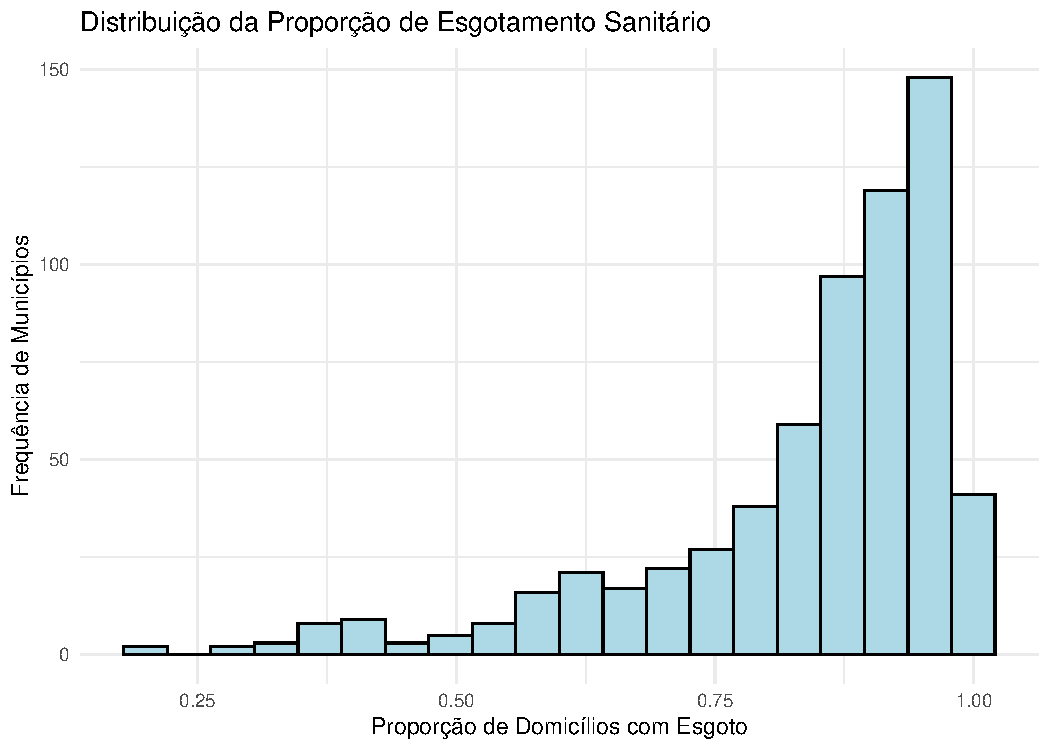
\includegraphics[width=0.7\textwidth]{histograma_y.pdf}
    %\framebox{\parbox{0.7\textwidth}{\centering\vspace{2cm}\textbf{01\_histograma\_y.pdf}\vspace{2cm}}}
    \caption{Distribuição da proporção de esgotamento sanitário nos municípios de São Paulo.}
    \label{fig:histograma}
\end{figure}

Ao observar a Figura \ref{fig:histograma}, nota-se que a distribuição empírica da proporção de esgoto é fortemente assimétrica à esquerda (ou negativa), como a diferença entre média e mediana indicou. A maioria dos municípios estão acima de $0,80$, formando uma cauda longa em direção aos valores mais baixos. Este comportamento distribucional assimétrico e o fato de a variável estar estritamente delimitada no intervalo contínuo $(0, 1)$ impossibilitam o uso de modelos lineares tradicionais baseados na suposição de normalidade, justificando a adoção do modelo de Regressão Beta.

Para explorar as relações entre a variável resposta e os preditores, construiu-se um painel de dispersão (Figura \ref{fig:painel_dispersao}).

% --- B. Painel de Dispersão (Juntando p1, p2, p3 e p4) ---
\begin{figure}[H]
    \centering
    \begin{subfigure}[b]{0.48\textwidth}
        \centering
        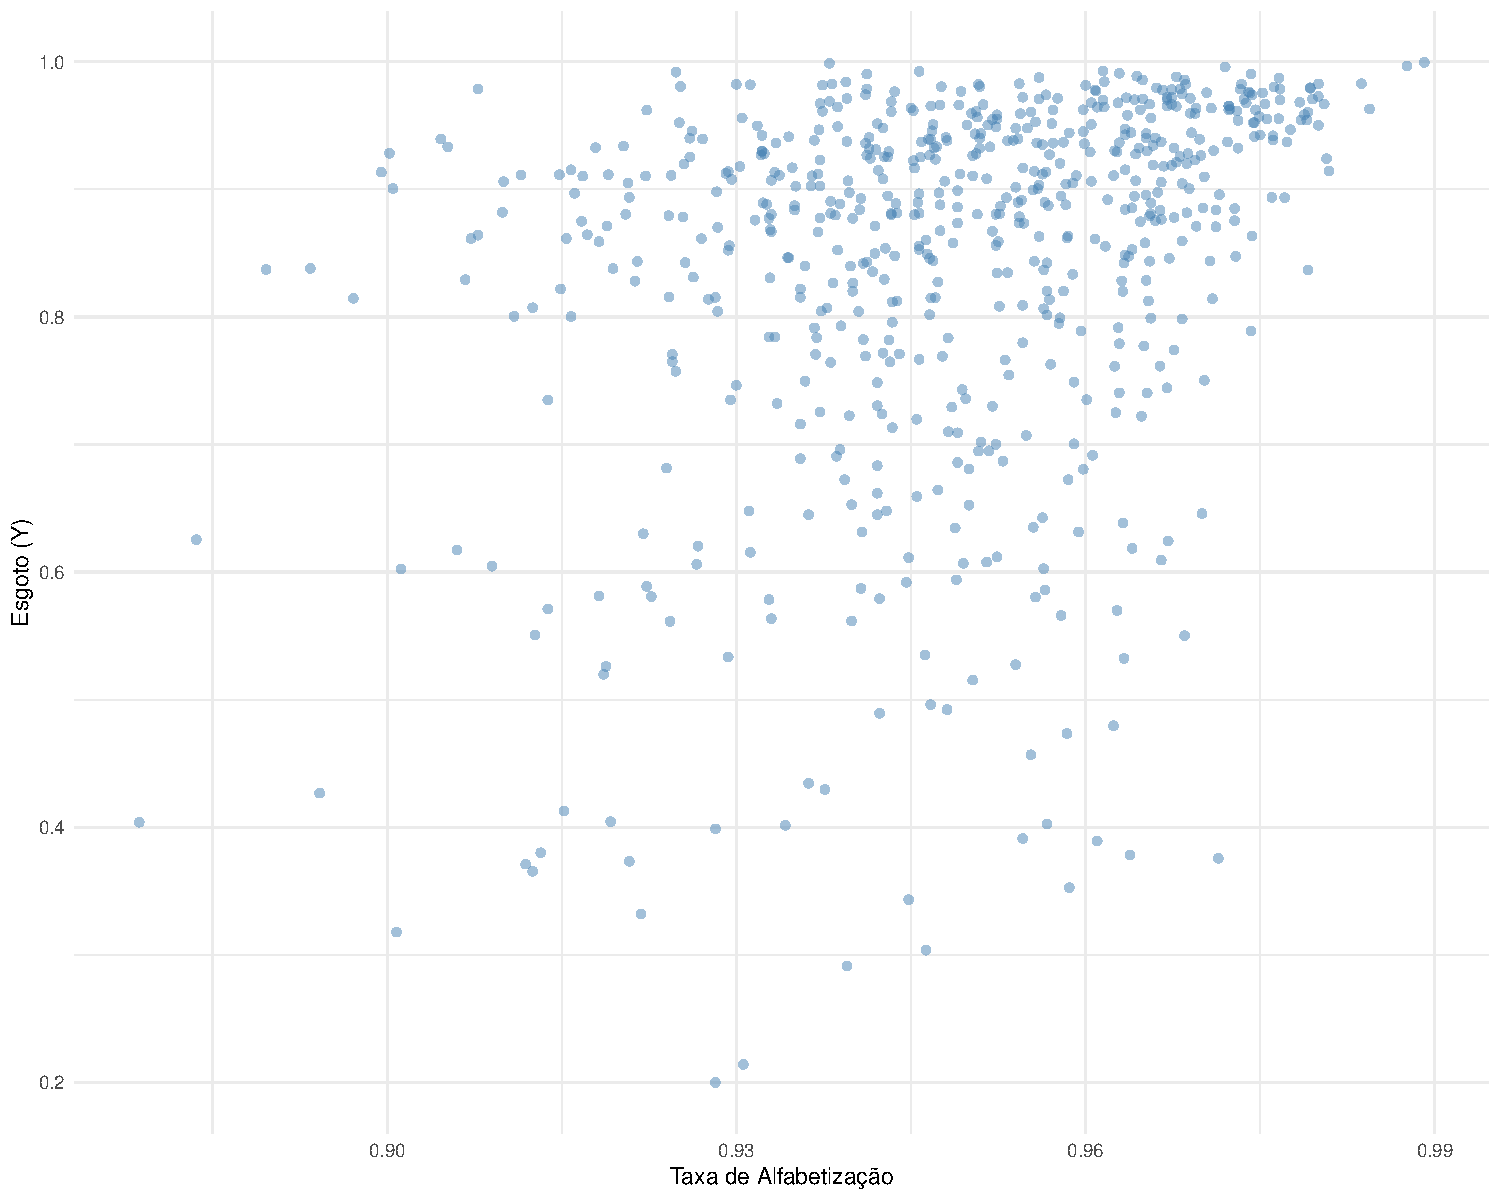
\includegraphics[width=\textwidth]{p1.pdf}
        %\framebox{\parbox{\textwidth}{\centering\vspace{1.5cm}\textbf{p1.pdf}\vspace{1.5cm}}}
        \caption{Alfabetização vs. Esgoto}
        \label{fig:p1}
    \end{subfigure}
    \hfill
    \begin{subfigure}[b]{0.48\textwidth}
        \centering
        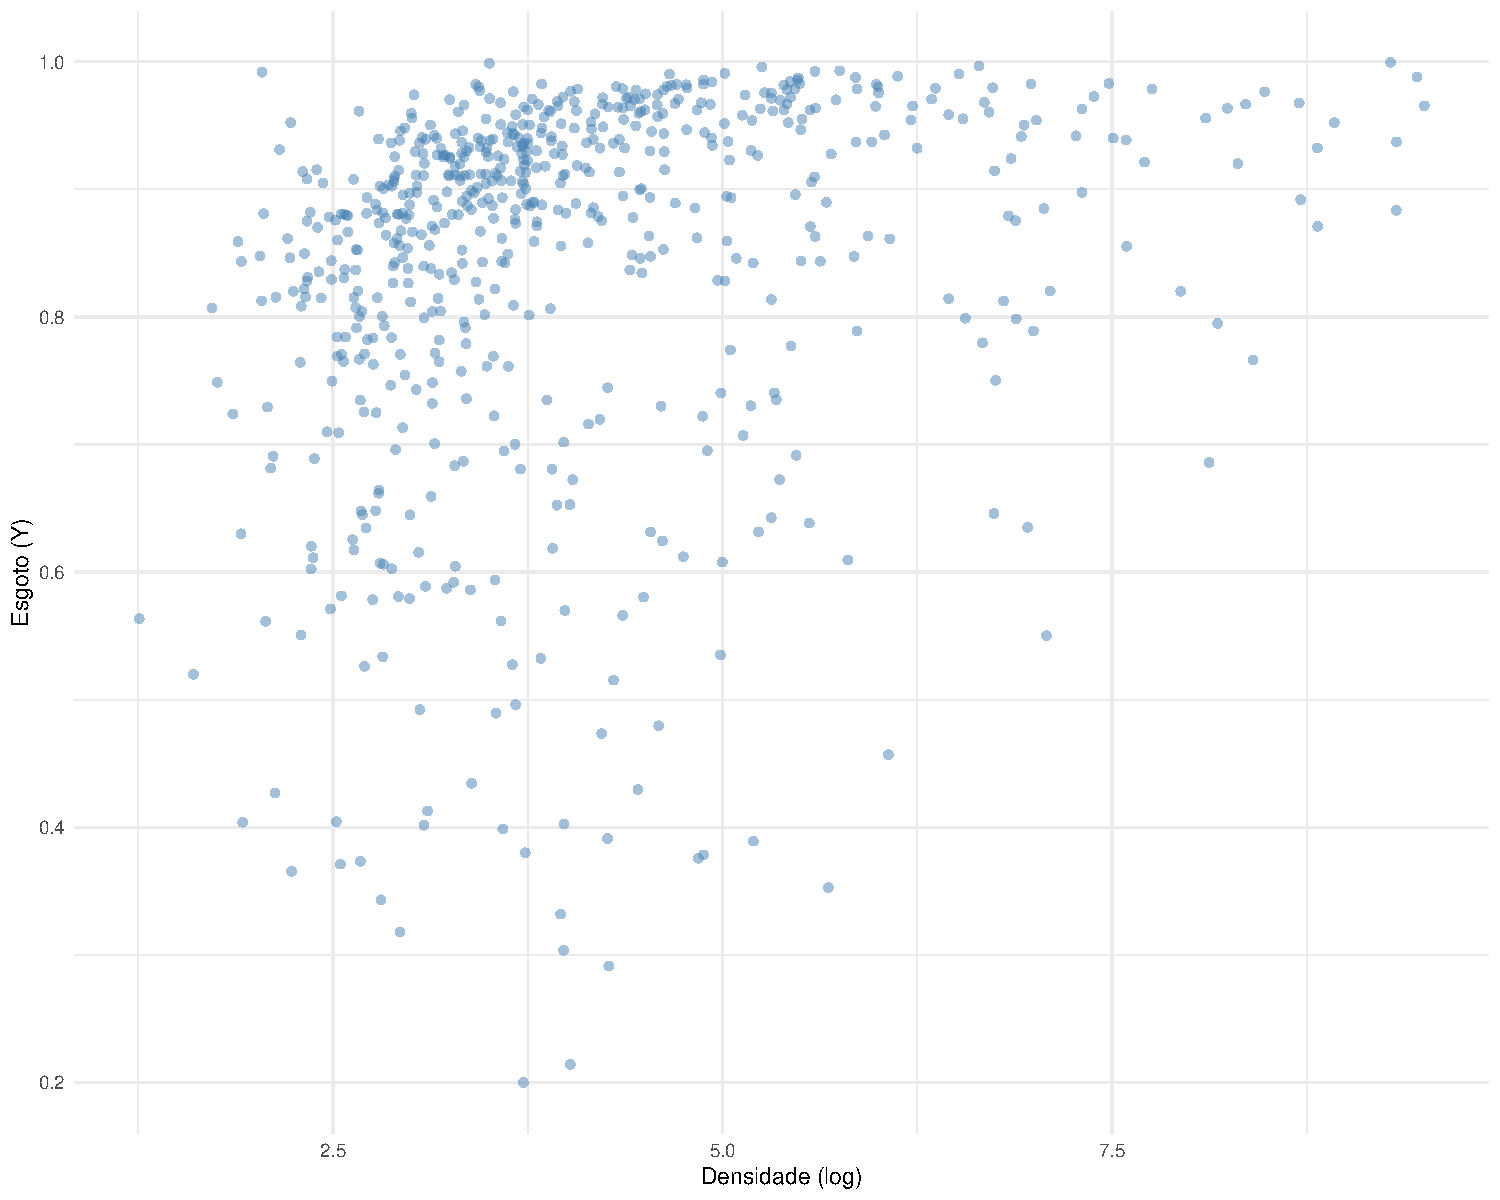
\includegraphics[width=\textwidth]{p2.pdf}
        %\framebox{\parbox{\textwidth}{\centering\vspace{1.5cm}\textbf{p2.pdf}\vspace{1.5cm}}}
        \caption{Densidade (log) vs. Esgoto}
        \label{fig:p2}
    \end{subfigure}
    
    \vspace{0.5cm} % Espaço entre as linhas
    
    \begin{subfigure}[b]{0.48\textwidth}
        \centering
        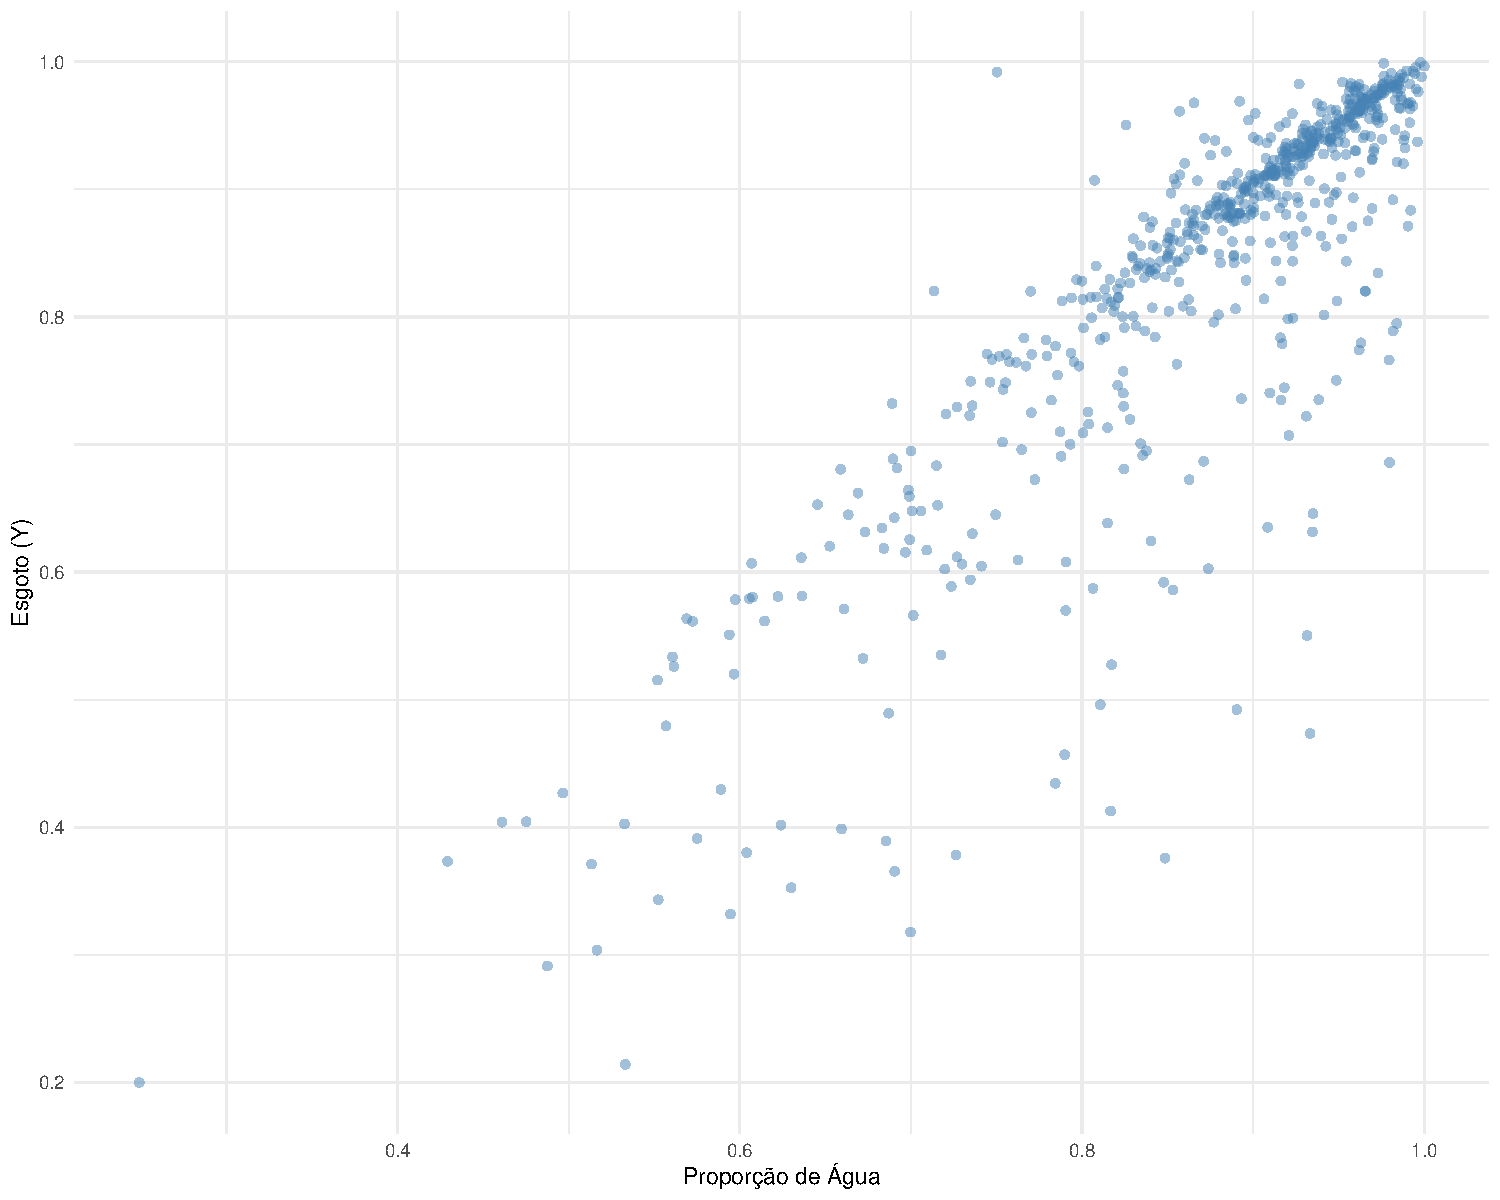
\includegraphics[width=\textwidth]{p3.pdf}
        %\framebox{\parbox{\textwidth}{\centering\vspace{1.5cm}\textbf{p3.pdf}\vspace{1.5cm}}}
        \caption{Água vs. Esgoto}
        \label{fig:p3}
    \end{subfigure}
    \hfill
    \begin{subfigure}[b]{0.48\textwidth}
        \centering
        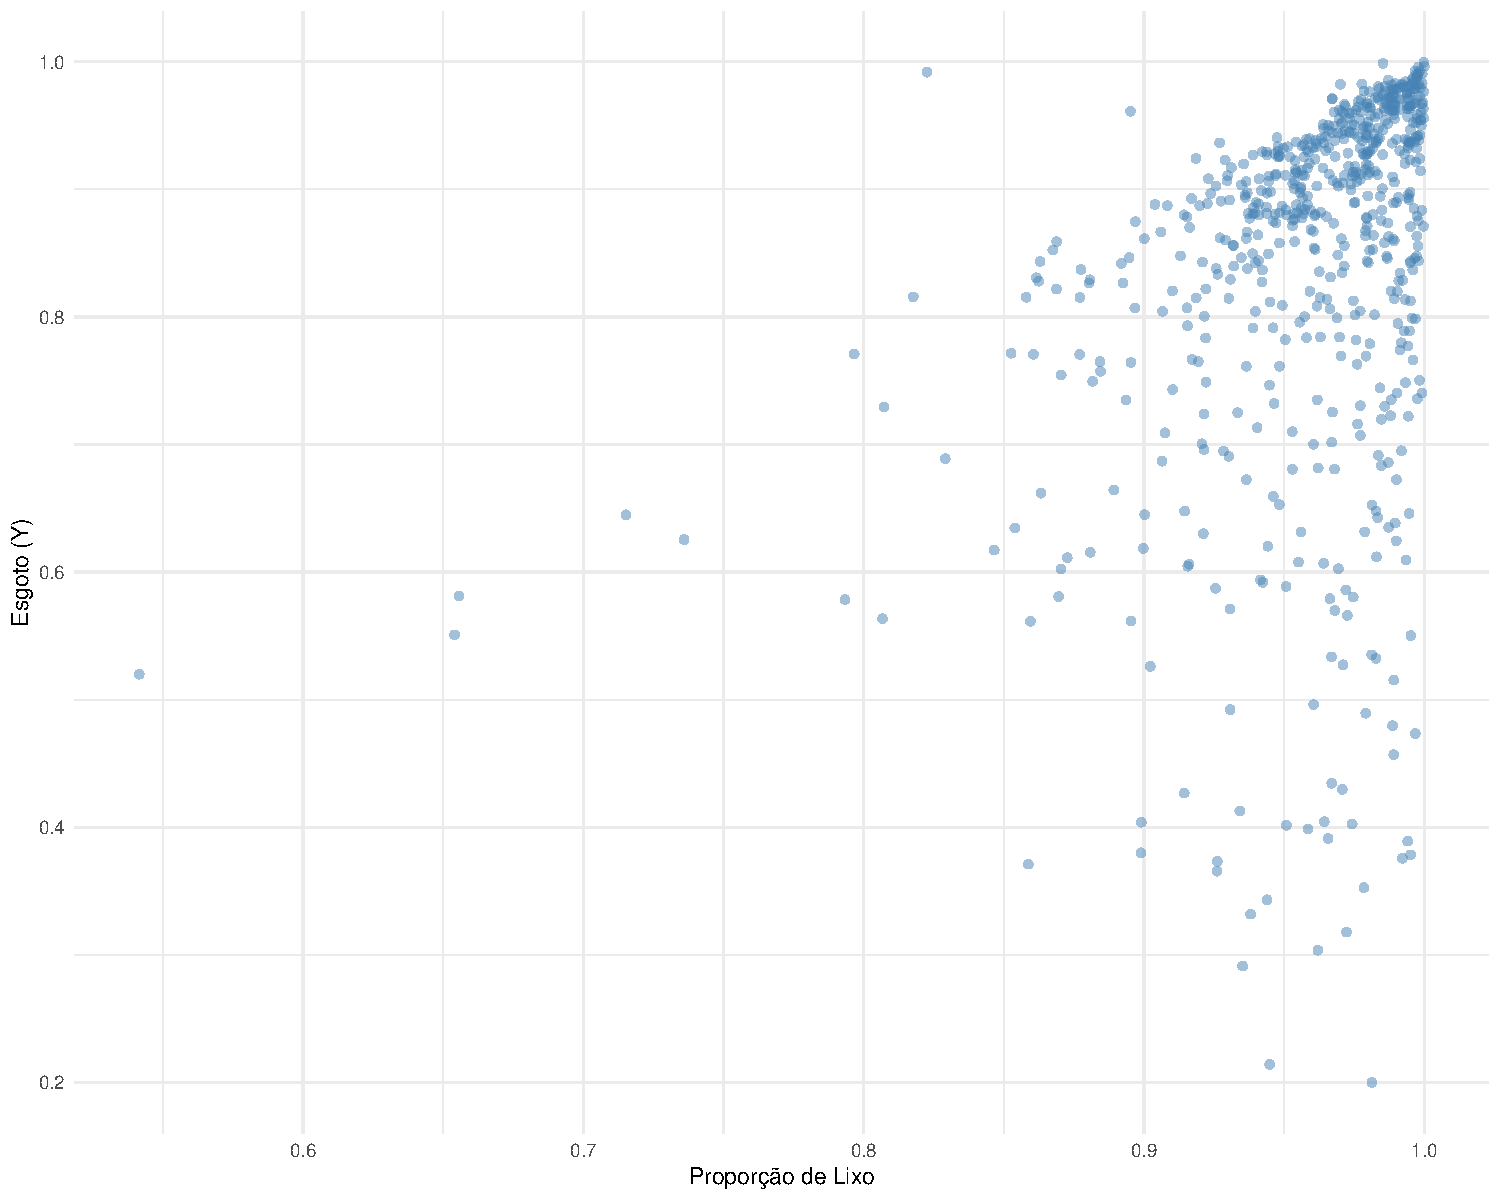
\includegraphics[width=\textwidth]{p4.pdf}
        %\framebox{\parbox{\textwidth}{\centering\vspace{1.5cm}\textbf{p4.pdf}\vspace{1.5cm}}}
        \caption{Lixo vs. Esgoto}
        \label{fig:p4}
    \end{subfigure}
    
    \caption{Painel de dispersão ilustrando a relação bivariada entre as covariáveis e a proporção de esgoto.}
    \label{fig:painel_dispersao}
\end{figure}

Visualmente, a variável que apresenta a relação linear mais nítida e positiva com o esgotamento sanitário é a proporção de abastecimento de água (Painel c). As demais covariáveis contínuas, como alfabetização (Painel a) e proporção de coleta de lixo (Painel d), apresentam uma maior dispersão, concentrando os dados no quadrante superior direito, o que reflete a correlação positiva esperada em infraestruturas urbanas interligadas. A densidade demográfica logaritmizada (Painel b) apresenta uma nuvem de pontos difusa, sugerindo que o seu efeito pode ser influenciado por outras dinâmicas espaciais.

A avaliação do componente espacial, por ser uma variável binária, foi relacionada com a  cobertura de esgoto entre os municípios do Interior em um boxplot (Figura \ref{fig:boxplot}).  

% --- C. Boxplot da Região Metropolitana ---
\begin{figure}[H]
    \centering
    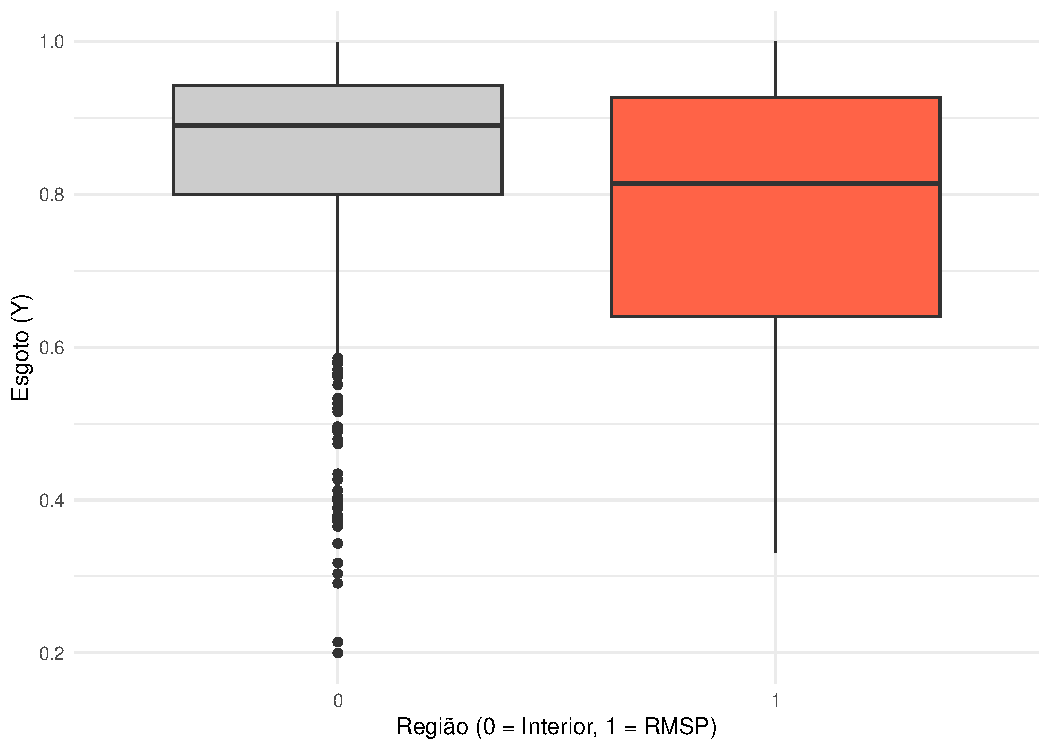
\includegraphics[width=0.75\textwidth]{boxplot_rmsp.pdf}
    %\framebox{\parbox{0.7\textwidth}{\centering\vspace{2cm}\textbf{03\_boxplot\_rmsp.pdf}\vspace{2cm}}}
    \caption{Cobertura de esgoto comparando municípios do Interior e da Região Metropolitana (RMSP).}
    \label{fig:boxplot}
\end{figure}

O boxplot evidencia que os municípios do interior (região $0$) possuem uma mediana de cobertura de esgoto visivelmente superior e um intervalo interquartílico mais compacto em comparação à RMSP (região $1$), cuja mediana situa-se acima de $0,80$ e apresenta uma dispersão interna muito mais acentuada. Não obstante, a caixa referente ao interior concentra uma extensa quantidade de outliers inferiores, representando provavelmente municípios rurais ou pequenos núcleos urbanos com déficits severos de saneamento (atingindo valores próximos a $0,20$). A RMSP embora não possua valores mínimos tão drásticos quanto o interior, tem a variação da sua cobertura assimétrica entre os centros urbanos e as suas periferias em expansão.

% --- D. Matriz de Correlação ---
\begin{figure}[H]
    \centering
    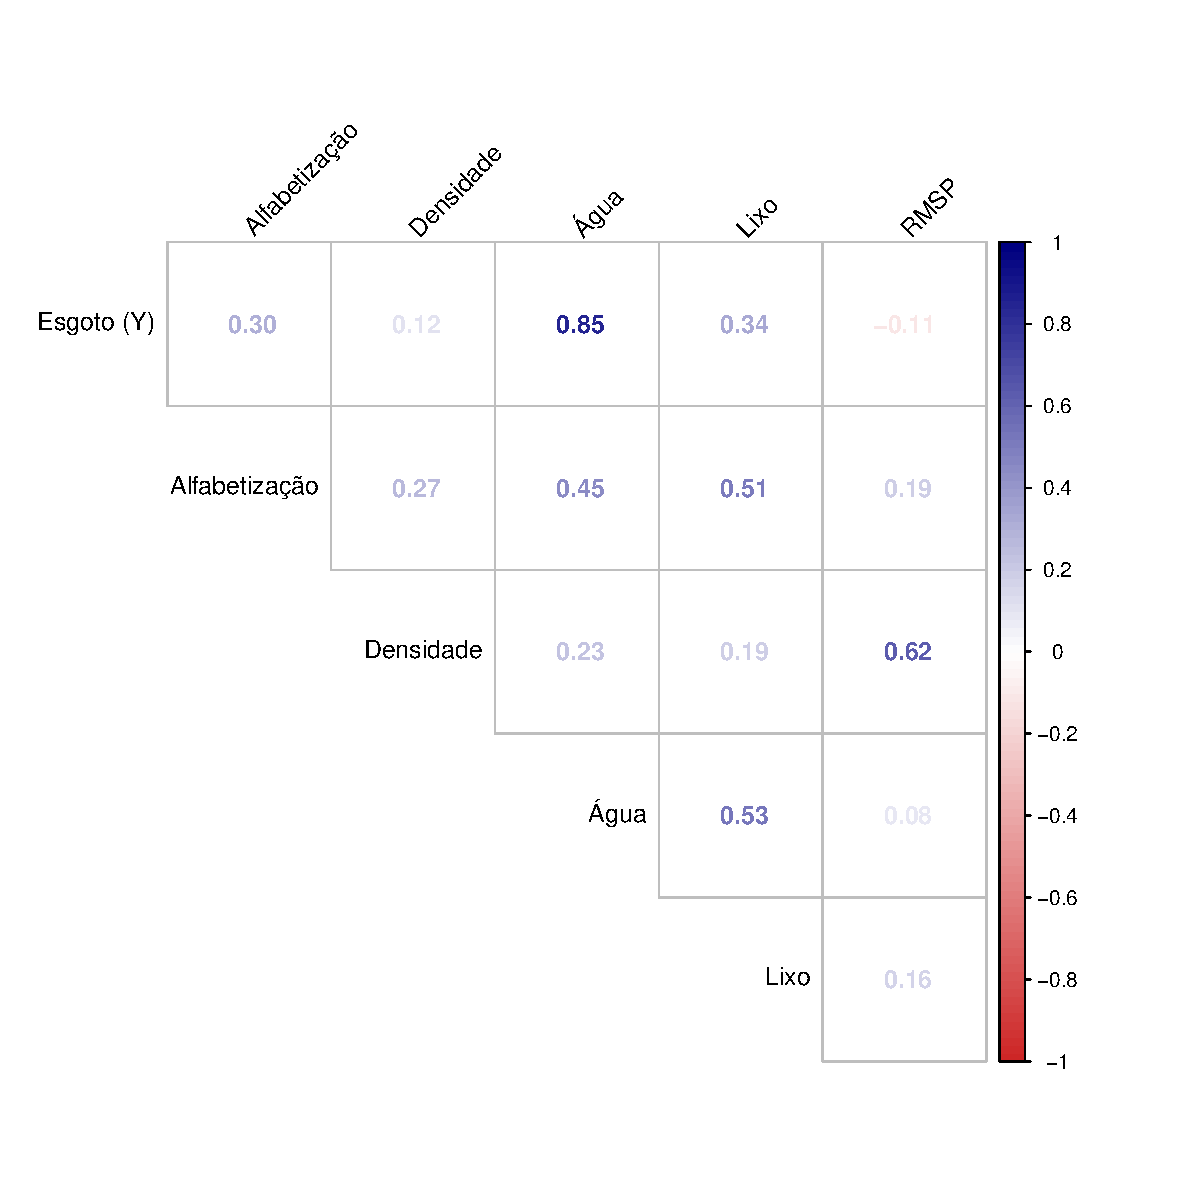
\includegraphics[width=0.75\textwidth]{matriz_correlacao.pdf}
    %\framebox{\parbox{0.75\textwidth}{\centering\vspace{2cm}\textbf{04\_matriz\_correlacao.pdf}\vspace{2cm}}}
    \caption{Matriz de correlação de Pearson entre as variáveis do estudo.}
    \label{fig:correlacao}
\end{figure}

A matriz de correlação de Pearson (Figura \ref{fig:correlacao}) quantifica as observações da Figura \ref{fig:painel_dispersao}. A associação linear positiva entre a proporção de água e a de esgoto é extremamente forte ($r = 0,85$). As correlações do esgoto com a alfabetização ($r = 0,30$) e com o lixo ($r = 0,34$) são de magnitude moderada. No que tange à multicolinearidade entre as variáveis explicativas, a maior correlação observada ocorreu entre a indicadora da Região Metropolitana de São Paulo (RMSP) e a densidade demográfica ($r = 0,62$), o que é sociologicamente esperado. Como nenhuma das correlações entre covariáveis ultrapassou limites críticos, o risco de multicolinearidade severa é mínimo, assegurando a estabilidade das estimativas do modelo.

% RESULTADOS
\section{Resultados}

\subsection{Seleção do Modelo}

A seleção do modelo ocorreu via método Forward Selection. O algoritmo Forward decide se continua a adicionar variáveis avaliando se há melhoria no critério de informação. s critérios utilizados foram o Akaike Information Criterion (AIC), Bayesian Information Criterion (BIC), Log-Likelihood (LL) e Pseudo R². A Tabela \ref{tab:selecao_modelos} apresenta a comparação dos modelos.

% --- TABELA 1: SELEÇÃO DE MODELOS ---
\begin{table}[H]
\centering
\caption{Comparação do ajuste dos modelos de Regressão Beta através de Critérios de Informação e Log-Verossimilhança.}
\label{tab:selecao_modelos}
\begin{tabular}{lrrrrr}
\toprule
\textbf{Modelo} & \textbf{Variáveis} & \textbf{AIC} & \textbf{BIC} & \textbf{Log-Likelihood} & \textbf{Pseudo $R^2$} \\
\midrule
M0: Modelo Nulo         & 0 & $-1054,38$ & $-1045,45$ & $529,2$ & -- \\
M1: Alfabetização       & 1 & $-1119,73$ & $-1106,32$ & $562,9$ & $0,1217$ \\
M2: + Densidade         & 2 & $-1129,46$ & $-1111,59$ & $568,7$ & $0,1411$ \\
M3: + Água              & 3 & $-1803,56$ & $-1781,21$ & $906,8$ & $0,6399$ \\
M4: + Lixo              & 4 & $-1806,63$ & $-1779,81$ & $909,3$ & $0,6400$ \\
\textbf{M5: Completo}   & \textbf{5} & $\mathbf{-1827,57}$ & $\mathbf{-1796,28}$ & $\mathbf{920,8}$ & $\mathbf{0,6594}$ \\
\bottomrule
\end{tabular}
\end{table}

O modelo nulo (M0), contendo apenas o intercepto, apresentou AIC de -1054,38 e BIC de -1045,45, servindo como referência para avaliação dos modelos subsequentes. A incorporação de Alfabetização (M1) resultou em melhora limitada dos critérios de seleção. A adição de Log Densidade (M2) manteve performance semelhante à M1. Contudo, a inclusão de Água (M3) representou um ponto de importante, com redução substancial do AIC para -1803,56 e aumento do Pseudo R² para 0,6399, indicando ganho explicativo significativo.

O modelo M4, que incluiu Lixo como preditor adicional, manteve performance ligeiramente melhor (AIC = -1806,63), enquanto M5, o modelo completo com todas as cinco variáveis independentes, apresentou os melhores critérios de ajuste com AIC = -1827,57 e BIC = -1796,28 e Pseudo R² = 0,6594. O Pseudo-$R^2$ padrão do modelo (baseado no quadrado da correlação entre o preditor linear e a resposta transformada) indicou um valor de 0,6594. De forma complementar, calculou-se o Pseudo-$R^2$ de Cox-Snell, que atingiu a marca de 0,7031. Estas métricas revelam que o modelo explica aproximadamente entre 65\% a 70\% da variabilidade na proporção de cobertura de esgoto, demonstrando adequação do modelo aos dados, principalmente considerando a extrema heterogeneidade entre metrópoles e municípios rurais. 

Para avaliar a significância global do modelo de Regressão Beta proposto em relação a um modelo nulo (contendo apenas o intercepto), também foi usado o Teste da Razão de Verossimilhança, cuja estatística é baseada na diferença das log-verossimilhanças (Deviance). O teste retornou uma estatística $\chi^2$ de 783,23 com 5 graus de liberdade, resultando num p-valor altamente significativo (p < 0,0001). Este resultado fornece evidências estatísticas robustas de que o conjunto de covariáveis selecionadas (abastecimento de água, coleta de lixo, densidade demográfica, alfabetização e a indicadora da RMSP) melhora a capacidade do modelo em explicar a proporção de esgotamento sanitário nos municípios. Consequentemente, o modelo completo foi selecionado para as próximas análises.

\subsection{Coeficientes Estimados}

A Tabela \ref{tab:coeficientes} apresenta as estimativas dos coeficientes do modelo de regressão beta completo e o p-valor do Teste Wald, obtidos após padronização das variáveis independentes. As variáveis foram padronizadas (média = 0, desvio padrão = 1) para permitir comparação direta da magnitude relativa dos efeitos e facilitar a interpretação em termos de mudanças por desvio padrão.

% --- TABELA 2: COEFICIENTES ---
\begin{table}[H]
\centering
\caption{Estimativas dos parâmetros do modelo de Regressão Beta para a proporção de esgotamento sanitário.}
\label{tab:coeficientes}
\begin{tabular}{lrrrr}
\toprule
\textbf{Parâmetro} & \textbf{Estimativa} & \textbf{Erro Padrão} & \textbf{IC 95\%} & \textbf{p-valor} \\
\midrule
Intercepto ($\beta_0$) & $1,825$  & $0,025$ & $[1,777; 1,873]$   & $<0,001$ \\
Alfabetização ($X_1$)  & $0,008$  & $0,031$ & $[-0,052; 0,069]$  & $0,782$ \\
Log Densidade ($X_2$)  & $0,020$  & $0,040$ & $[-0,058; 0,097]$  & $0,621$ \\
Água ($X_3$)           & $0,818$  & $0,024$ & $[0,770; 0,865]$   & $<0,001$ \\
Lixo ($X_4$)           & $-0,062$ & $0,024$ & $[-0,109; -0,015]$ & $0,009$ \\
RMSP ($X_5$)           & $-0,139$ & $0,027$ & $[-0,192; -0,087]$ & $<0,001$ \\
\midrule
Precisão ($\phi$)      & $23,079$ & $1,293$ & $[20,544; 25,614]$ & $<0,001$ \\
\bottomrule
\end{tabular}
\end{table}

Entre as variáveis significativas, a variável Água ($\beta = 0,818$, $p < 0,001$) apresentou o efeito mais forte, com intervalo de confiança de 95\% $[0,770; 0,865]$ inteiramente acima de zero. RMSP ($\beta = -0,139$, $p < 0,001$) também demonstrou significância estatística, com efeito negativo e intervalo de confiança $[-0,192; -0,087]$. A variável Lixo ($\beta = -0,062$, $p = 0,009$) mostrou significância marginal com intervalo $[-0,109; -0,015]$, indicando efeito protetor, embora de menor magnitude que as demais.

As variáveis Alfabetização ($\beta = 0,008$, $p = 0,782$) e Log Densidade ($\beta = 0,020$, $p = 0,621$) não apresentaram efeitos estatisticamente significativos, com intervalos de confiança incluindo zero $[−0,052; 0,069]$ e $[−0,058; 0,097]$, respectivamente. Esses resultados sugerem que, após controle pelas demais variáveis, alfabetização e densidade populacional não explicam variação significativa na cobertura de esgoto.

O intercepto ($\beta_0 = 1,825$, $p < 0,001$) representa o valor predito quando todas as variáveis independentes estão em suas médias originais. O parâmetro de precisão ($\phi = 23,079$, $p < 0,001$) é estatisticamente significativo e indica boa precisão do ajuste..

\subsection{Razão de Chances}

Na regressão beta, a razão de chances ($OR = e^\beta$) ferecem interpretação mais intuitiva dos efeitos estimados, representando mudanças multiplicativas na proporção esperada para cada aumento de um desvio padrão nas variáveis independentes. A Tabela \ref{tab:odds_ratios} apresenta os valores de OR com seus respectivos intervalos de confiança de 95\%.

% --- TABELA 3: ODDS RATIOS ---
\begin{table}[H]
\centering
\caption{Razões de Chances (OR) e Intervalos de Confiança (IC 95\%) do modelo de Regressão Beta.}
\label{tab:odds_ratios}
\begin{tabular}{lrr}
\toprule
\textbf{Parâmetro} & \textbf{OR ($e^\beta$)} & \textbf{IC 95\% (OR)} \\
\midrule
Intercepto ($\beta_0$) & $6,2006$ & $[5,9092; 6,5064]$ \\
Alfabetização ($X_1$)  & $1,0085$ & $[0,9496; 1,0712]$ \\
Log Densidade ($X_2$)  & $1,0198$ & $[0,9434; 1,1024]$ \\
Água ($X_3$)           & $2,2654$ & $[2,1600; 2,3760]$ \\
Lixo ($X_4$)           & $0,9398$ & $[0,8968; 0,9848]$ \\
RMSP ($X_5$)           & $0,8699$ & $[0,8253; 0,9169]$ \\
\bottomrule
\end{tabular}
\end{table}

A variável Água apresenta a razão de chances mais elevada (OR = 2,2654, IC95\%: [2,1600; 2,3760]), indicando que um aumento de um desvio padrão nesta variável está associado com uma multiplicação de aproximadamente 2,27 vezes na proporção esperada de cobertura de esgoto. Este é o preditor mais determinante para explicar a variação em cobertura de esgoto.

O indicador de região metropolitana (RMSP), apresenta razão de chances abaixo de um (OR = 0,8699, IC95\%: [0,8253; 0,9169]), indicando efeito protetor. Aumentos de um desvio padrão em RMSP estão associados com redução de aproximadamente 13\% (100\% × [1 − 0,8699]) na proporção esperada de cobertura de esgoto. Este é um efeito de magnitude considerável e estatisticamente significativo, assim como a variável Lixo com razão de chances também abaixo de um (OR = 0,9398, IC95\%: [0,8968; 0,9848]), sugerindo efeito protetor de menor magnitude que RMSP. Um aumento de um desvio padrão em Lixo está associado com redução de aproximadamente 6\% na proporção de cobertura de esgoto.

Alfabetização ($X_1$) e Log Densidade ($X_2$): Ambas apresentam razões de chances muito próximas a um (OR = 1,0085 e OR = 1,0198, respectivamente), com intervalos de confiança incluindo 1. Estes resultados confirmam a ausência de significância estatística e efeitos práticos negligenciáveis dessas variáveis.

\subsection{Diagnóstico de Multicolinearidade}

Para avaliar a presença de multicolinearidade entre as variáveis explicativas, calculou-se o Fator de Inflação da Variância (VIF) para cada preditor, cujos resultados estão na Tabela \ref{tab:vif}.

% --- TABELA 4: VIF ---
\begin{table}[H]
\centering
\caption{Diagnóstico de multicolinearidade através do Fator de Inflação da Variância (VIF).}
\label{tab:vif}
\begin{tabular}{lr}
\toprule
\textbf{Variável} & \textbf{VIF} \\
\midrule
Alfabetização ($X_1$) & $1,995$ \\
Log Densidade ($X_2$) & $3,115$ \\
Água ($X_3$)          & $1,538$ \\
Lixo ($X_4$)          & $1,732$ \\
RMSP ($X_5$)          & $1,605$ \\
\bottomrule
\end{tabular}
\end{table}

Na literatura estatística, valores de VIF superiores a 5 (ou 10, num limiar menos conservador) são indicadores de colinearidade severa, o que pode inflacionar os erros padrão e instabilizar as estimativas do modelo. Conforme observado na Tabela \ref{tab:vif}, todas as variáveis apresentaram valores de VIF confortavelmente abaixo do limite crítico de 5, situando-se entre $1,538$ (Água) e $3,115$ (Log Densidade). Estes resultados indicam a ausência de problemas de multicolinearidade, garantindo que os efeitos individuais de cada covariável sociodemográfica e de infraestrutura sobre a proporção de esgoto puderam ser estimados com estabilidade e precisão.

\subsection{Análise dos Resíduos}

A Tabela \ref{tab:residuos} apresenta as estatísticas descritivas dos resíduos Deviance e Pearson do modelo ajustado. Ambos os tipos de resíduos são apropriados para diagnóstico em modelos de regressão beta, sendo preferível a análise de resíduos Deviance devido a sua melhor aproximação com distribuições-padrão.

% --- TABELA 5: RESÍDUOS ---
\begin{table}[H]
\centering
\caption{Estatísticas descritivas e teste de normalidade dos resíduos do modelo.}
\label{tab:residuos}
\begin{tabular}{lrrrrr}
\toprule
\textbf{Resíduo} & \textbf{Média} & \textbf{Mín.} & \textbf{Máx.} & \textbf{Desv. Pad.} & \textbf{p-valor (KS)} \\
\midrule
Deviance & $-0,0080$ & $-4,6510$ & $5,1340$ & $0,9203$ & $< 0,001$ \\
Pearson  & $0,0700$ & $-7,2923$ & $3,2218$ & $1,0788$ & $< 0,001$ \\
\bottomrule
\end{tabular}
\end{table}

Os resíduos Deviance apresentaram média de −0,0080, muito próxima de zero como esperado em modelo bem ajustado. O desvio padrão de 0,9203 aproxima-se de um, indicando adequada padronização. A amplitude entre mínimo (−4,6510) e máximo (5,1340) sugere ausência de outliers extremos que pudessem comprometer o ajuste do modelo. Um comportamento análogo ocorre com os resíduos Pearson, apresentando média de 0,0700 e desvio padrão de 1,0788. A distribuição mostrou assimetria entre mínimo (−7,2923) e máximo (3,2218), padrão frequente em modelos beta quando há observações próximas aos limites do intervalo (0,1). O teste de Kolmogorov-Smirnov (KS) indicou desvio significativo de normalidade ($p < 0,001$) para ambos os tipos de resíduos. Essas mesmas observações são notórias analisando a Figura \ref{fig:residuos}. 

% --- E. Gráficos de Resíduos e Diagnóstico ---
\begin{figure}[H]
    \centering
    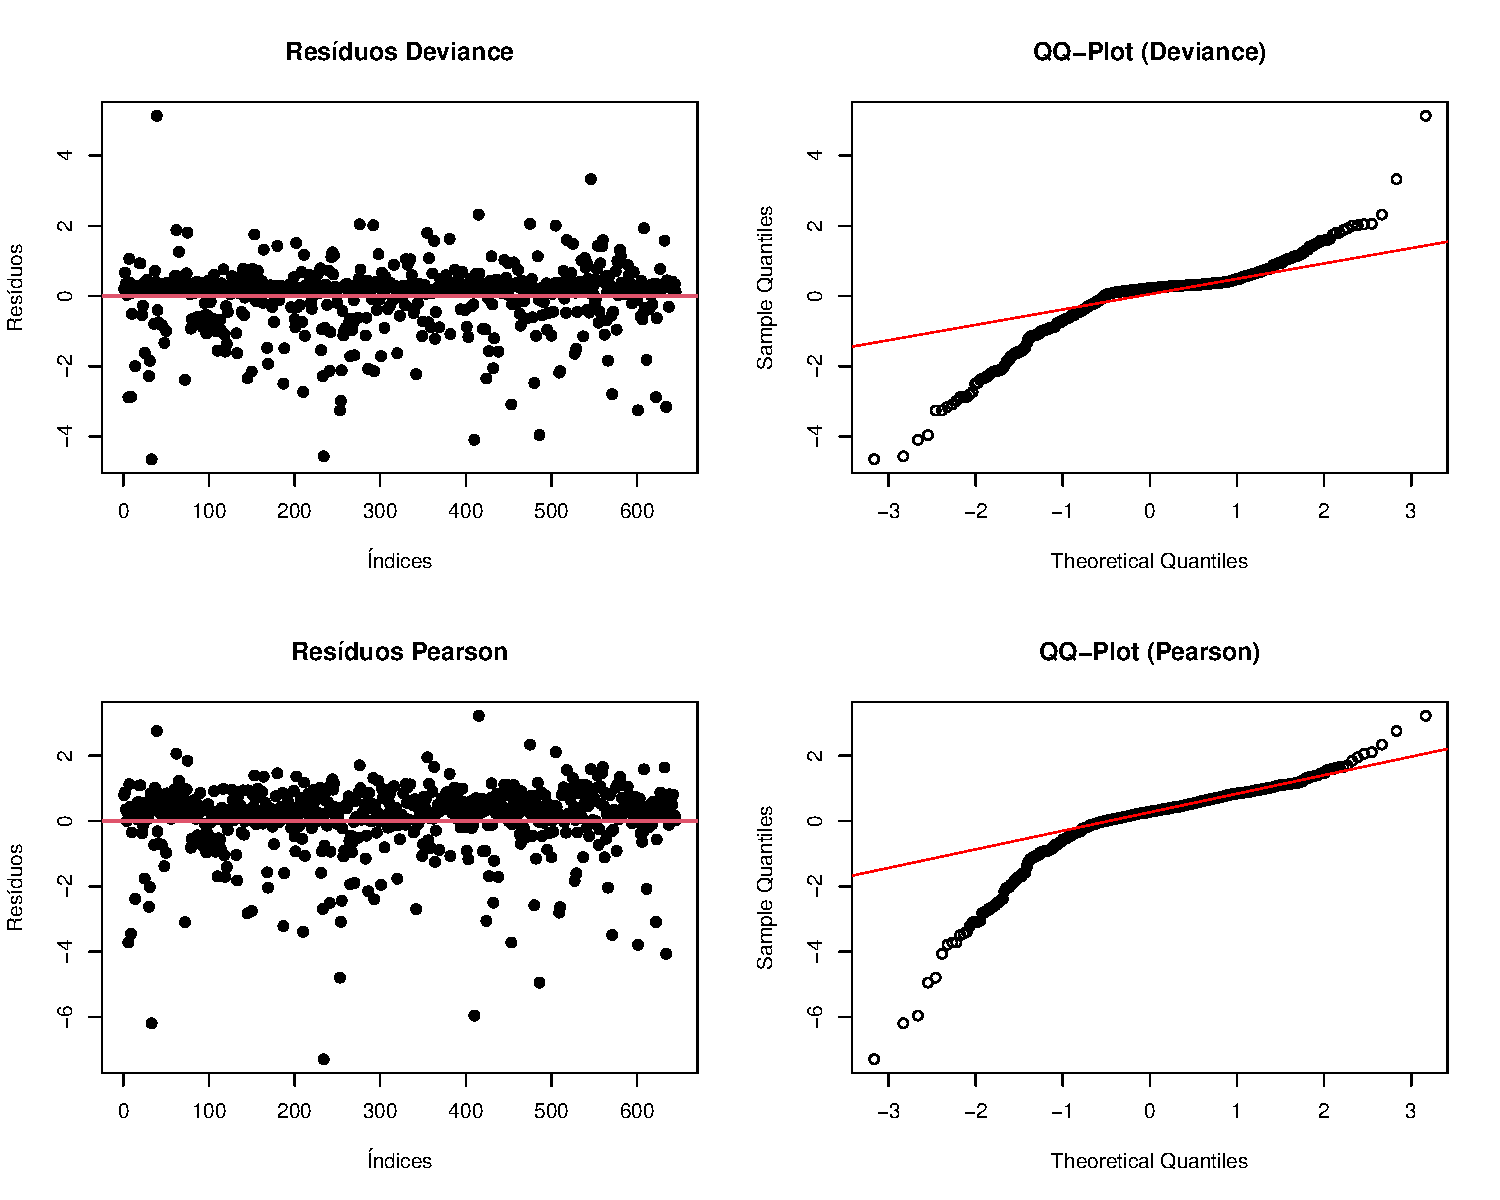
\includegraphics[width=0.9\textwidth]{graficos_residuos.pdf}
    %\framebox{\parbox{0.9\textwidth}{\centering\vspace{2cm}\textbf{05\_graficos\_residuos.pdf}\vspace{2cm}}}
    \caption{Análise de resíduos do modelo de Regressão Beta (Resíduos Deviance e Pearson).}
    \label{fig:residuos}
\end{figure}

A Figura \ref{fig:residuos} evidência a assimetria negativa dos resíduos Pearson e ambos QQ Plot mostram a não correspondência dos resíduos com a linha de referência (linha vermelha), indicando falta de normalidade como o Teste KS. Este resultado é esperado, uma vez que a distribuição condicional segue a família beta e não a normal. A estimação por máxima verossimilhança é boa a desvios de normalidade, não comprometendo a validade das inferências.

\subsection{Diagnóstico de Observações Influentes e Alavancagem}

As estimativas do modelo de Regressão Beta também foram avaliadas através do diagnóstico de observações atípicas, focando em três métricas: Distância de Cook (influência global), Curvatura Normal (influência local) e valores de hat (alavancagem), cujos resultados visuais encontram-se na Figura
\ref{fig:influencia}. 

% --- F. Medidas de Influência ---
\begin{figure}[H]
    \centering
    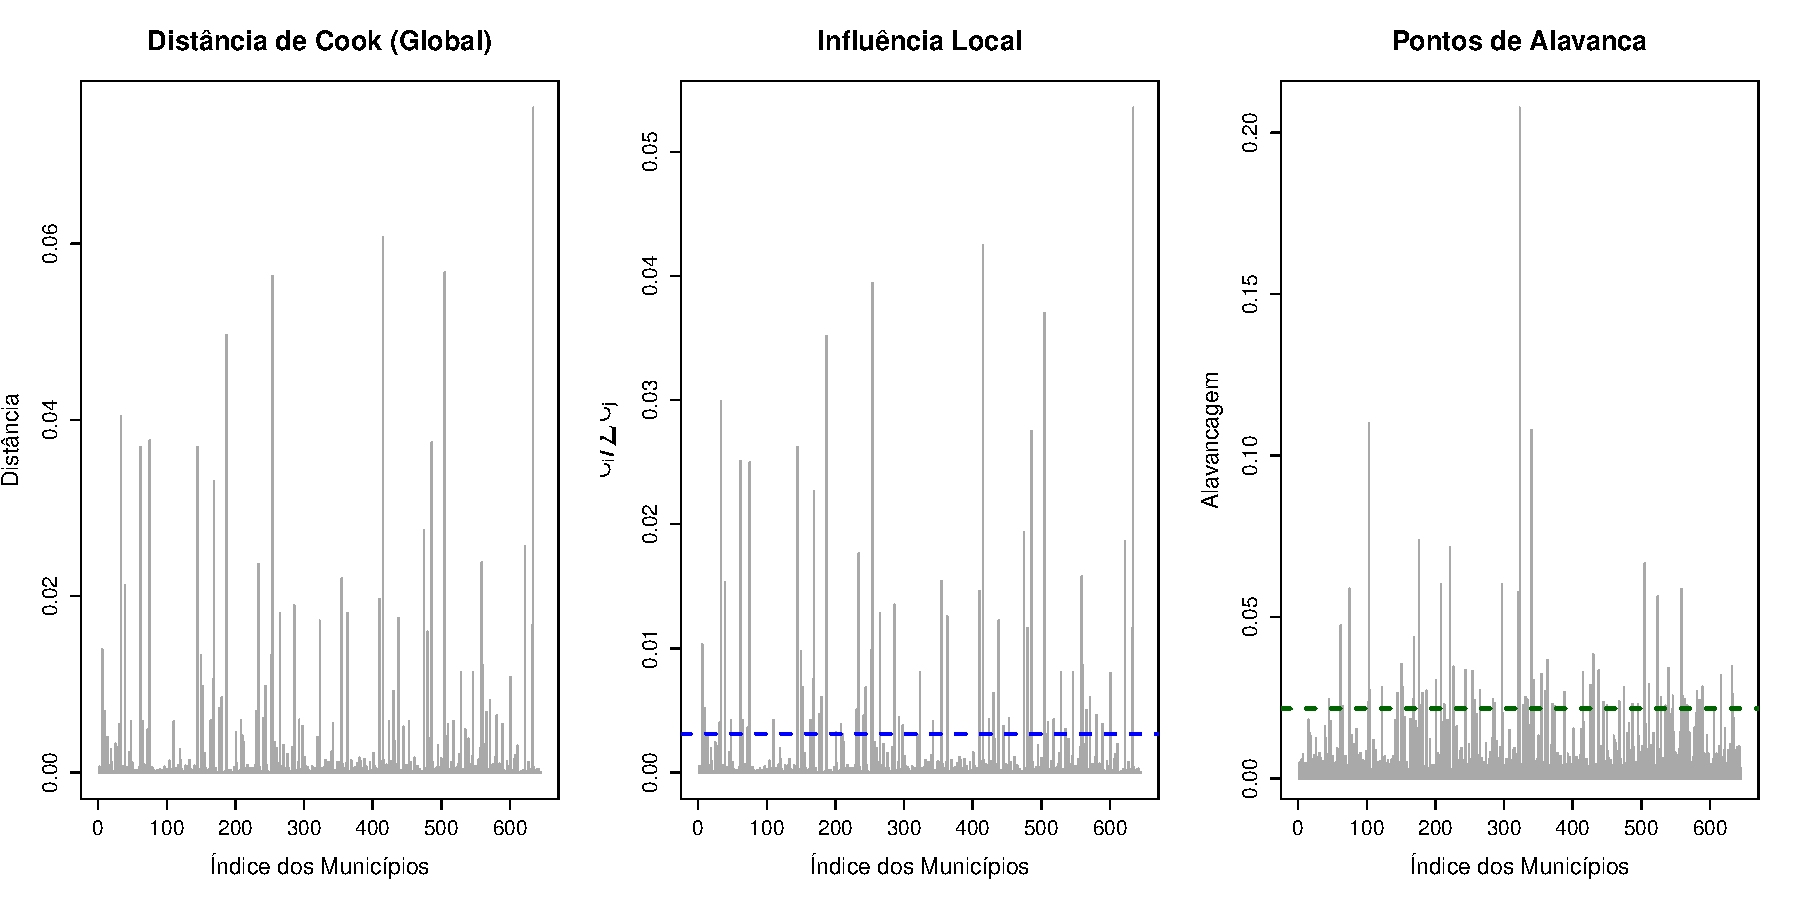
\includegraphics[width=0.9\textwidth]{graficos_influencia.pdf}
    %\framebox{\parbox{0.9\textwidth}{\centering\vspace{2cm}\textbf{06\_medidas\_influencia.pdf}\vspace{2cm}}}
    \caption{Gráficos de diagnóstico de observações influentes (Distância de Cook e Alavancagem).}
    \label{fig:influencia}
\end{figure}

A análise da Distância de Cook revelou um cenário de elevada estabilidade global. Nenhuma das observações atingiu o limiar crítico (geralmente estabelecido em $0,8$ ou $1,0$), indicando que não existe um único município que, isoladamente, dite a direção ou a magnitude dos coeficientes do modelo.

No entanto, o diagnóstico de Influência Local, que avalia a sensibilidade do modelo a pequenas perturbações no peso das observações, identificou 68 municípios (aproximadamente $10,5\%$ da amostra) acima do limite de $2\bar{C} = 0,0031$. Em paralelo, a análise de Pontos de Alavanca, focada em identificar municípios com valores extremos nas variáveis explicativas espaciais (alta/baixa densidade, infraestrutura extrema), sinalizou 73 municípios (cerca de $11,3\%$ da amostra) acima do ponto de corte de $2p/n = 0,0217$, onde $p=7$ é a quantidade de coeficientes do modelo.

Para compreender o impacto destas observações na estrutura do modelo, foi feita uma Análise de Sensibilidade, reestimando a regressão após a exclusão combinada destes pontos discrepantes (104 observações). Os resultados demonstraram que o parâmetro de precisão ($\phi$) saltou de $23,07$ para $53,77$, o que confirma que estes municípios são, de fato, os maiores responsáveis pela dispersão da variância na amostra.

O achado mais notável da análise de sensibilidade foi a alteração nas inferências: enquanto a variável de Abastecimento de Água ($X_3$) manteve a sua forte significância ($p < 0,001$), as variáveis de Coleta de Lixo ($X_4$) e a indicadora da RMSP ($X_5$) perderam a significância estatística (passando para $p = 0,559$ e $p = 0,347$, respetivamente).

A listagem das 104 observações identificados com alta influência local e/ou alavancagem está presente no Apêndice A. A Tabela \ref{tab:sumario_extremos} apresenta esses dados sumarizados.

\begin{table}[htbp]
\centering
\caption{Estatísticas descritivas do subgrupo de observações extremas e de alta alavancagem ($n = 104$).}
\label{tab:sumario_extremos}
\begin{tabular}{lrrrrrr}
\toprule
\textbf{Variável} & \textbf{Mín.} & \textbf{Q1} & \textbf{Mediana} & \textbf{Média} & \textbf{Q2} & \textbf{Máx.} \\
\midrule
Proporção de Esgoto & $0,1998$ & $0,4780$ & $0,6182$ & $0,6338$ & $0,8024$ & $0,9995$ \\
Densidade Demográfica & $3,51$ & $19,85$ & $79,94$ & $1336,21$ & $867,62$ & $13416,81$ \\
Coleta de Lixo & $0,5416$ & $0,9333$ & $0,9746$ & $0,9456$ & $0,9936$ & $0,9998$ \\
\bottomrule
\multicolumn{7}{l}{\footnotesize \textit{Nota:} Dos 104 municípios atípicos, 38 ($36,5\%$) pertencem à RMSP.}
\end{tabular}
\end{table}

A análise das estatísticas descritivas deste estrato (Tabela \ref{tab:sumario_extremos}) revela a singularidade da RMSP devido a sobrerrepresentação quase total da Região Metropolitana. Dos 104 municípios listados, 38 pertencem à RMSP. Considerando que a região metropolitana é constituída por um total de 39 municípios, conclui-se que $97,4\%$ do território metropolitano paulista apresenta um comportamento estatístico extremo, de alta alavancagem ou influência local em relação à tendência do interior do Estado. Este achado valida matematicamente a perda de significância da variável indicadora da RMSP quando estes pontos são excluídos na análise de sensibilidade.

Além disso, as estatísticas de densidade demográfica deste subgrupo espelham a dualidade da ocupação do solo em São Paulo. A amplitude da densidade é extrema, variando de ocupações puramente rurais ($3,51$ hab/km²) a hipercentros urbanos ($13.416,81$ hab/km²). A forte assimetria desta distribuição é evidenciada pela distância entre a mediana ($79,94$ hab/km²) e a média amostral ($1.336,21$ hab/km²). O modelo identificou corretamente que a variação no esgotamento sanitário é impulsionada justamente nos municípios extremamente rarefeitos (onde a rede de esgoto é inviável) e as metrópoles superadensadas (onde a rede é universalizada, mas lida com déficits de periferia).

Apesar da coleta de lixo apresentar uma cobertura ampla para a maioria do Estado (com mediana de $97,46\%$ neste subgrupo), a presença de municípios com taxas de recolha de resíduos sólidos de apenas $54,16\%$ sinaliza déficits infraestruturais que fogem ao padrão paulista. São estas assimetrias pontuais que conferem estabilidade ao coeficiente da coleta de lixo no modelo multivariado original.

Portanto, os 104 municípios sinalizados pelos diagnósticos de influência e alavancagem não representam ruídos estatísticos ou erros de amostragem, mas ocorrem devido as desigualdade do território de São Paulo, englobando a totalidade da Região Metropolitana e os extremos de densidade do interior. Consequentemente, a preservação do modelo com a amostra completa ($N=645$) reafirma-se como a abordagem mais correta e representativa para o estudo do esgotamento sanitário.

% CONCLUSÃO
\section{Conclusão}

O presente estudo teve como objetivo central modelar e estudar os componentes sociodemográficos e de infraestrutura que explicam a proporção de esgotamento sanitário nos 645 municípios do Estado de São Paulo. A escolha metodológica pela Regressão Beta demonstrou ser estatisticamente robusta em frente à assimetria de dados limitados ao intervalo $(0,1)$. O modelo final comprovou a sua adequação e robustez global através do Teste da Razão de Verossimilhança ($p < 0,0001$), alcançando um bom poder explicativo, traduzido por um Pseudo-$R^2$ de Cox-Snell de $0,7031$. Isto significa que o conjunto de variáveis selecionado é capaz de capturar cerca de $70\%$ de toda a variabilidade do saneamento no território paulista.

A análise inferencial das estimativas revelou que a expansão da rede de esgoto não ocorre num vazio urbano, estando junto à presença de outras infraestruturas básicas. O abastecimento de água foi o principal preditor, evidenciando que as obras de saneamento subterrâneo e de distribuição hídrica expandem-se de forma conjunta. Em contrapartida, fatores puramente sociais, como a taxa de alfabetização, não apresentaram significância estatística, sugerindo que a presença física da rede de esgoto é principalmente explicada por dinâmicas de engenharia urbana e densidade, e não pelo nível educacional da população.

A análise de diagnóstico de influência e alavancagem identificou 104 municípios com perfis estatísticos extremos, mas que não apontaram erros de amostragem ou digitação. Esses pontos de influencia mostraram a heterogeneidade do território paulista com que quase a totalidade da Região Metropolitana de São Paulo (RMSP) com polo de alavancagem indicando que a infraestrutura do Estado é moldada por extremos: os hipercentros e os municípios rurais. A constatação de que a remoção destes pontos faria variáveis como a indicadora da RMSP e a coleta de lixo perderem o seu efeito no modelo demonstra que a desigualdade. Homogeneizar a amostra excluindo estas observações significaria mascarar a realidade intrincada.

Por fim, as implicações práticas deste estudo indicam que as políticas públicas de saneamento devem ser integradas. O planeamento urbano e os investimentos estruturais não podem ignorar a coexistência paralela de serviços como água e esgoto, tampouco a pressão exercida pelos grandes adensamentos populacionais.

% REFERÊNCIAS
\newpage
\bibliography{ref}

\end{document}